En base a los anteriores requisitos el grupo de desarrollo ha generado los siguientes diagramas para el software de la placa de control.

Cabe destacar que los estados de error funcionan en cascada, es decir, dado que cada uno de los diagramas de estados representa una función del código, estas podrán tener errores en su ejecución y estos errores se irán propagando en cascada hacia niveles mas altos de abstracción a lo largo de las diferentes funciones que han sido invocadas.

\begin{figure}[H]
    \centering
    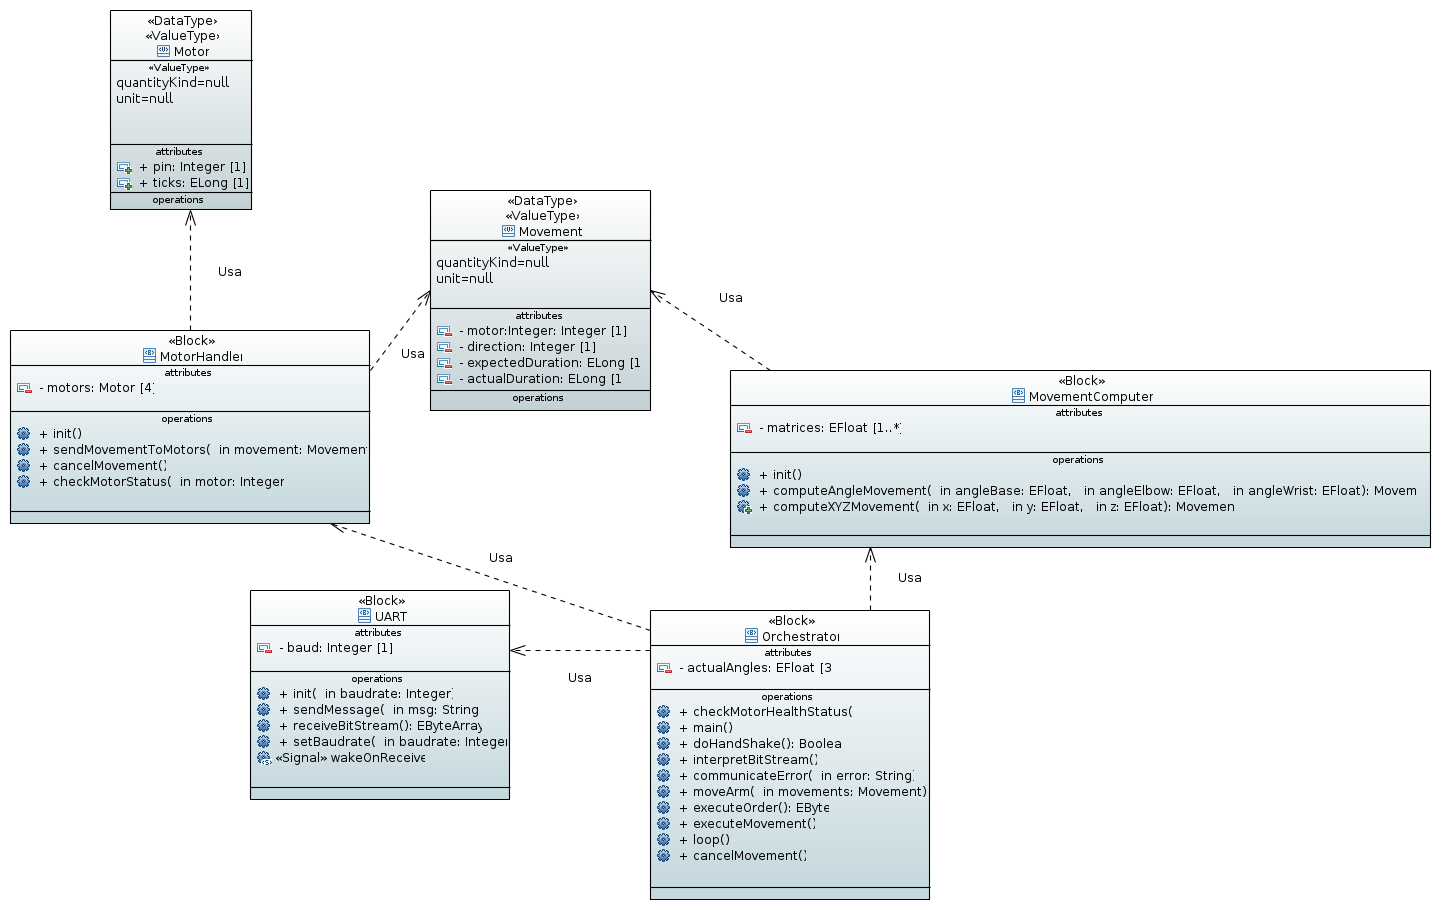
\includegraphics[width=\linewidth]{pictures/S2BlockDiagram.PNG}
    \caption{Diagrama de bloques de \ac{S2}}
    \label{fig:diagrama_bloques_s2}
\end{figure}

En el diagrama \ref{fig:diagrama_bloques_s2} se pueden observar los bloques que componen \ac{S2} además de dos tipos de datos los cuales han sido creados para facilitar el control de los motores del brazo.

A continuación se explican cada uno de los bloques:

\begin{itemize}
    \item \texttt{MotorHandler}: este bloque es capaz de controlar los motores de manera directa empleando el tipo de dato ``\texttt{Movement}'' enviando la señal necesaria para realizar el movimiento requerido. Además permite verificar el estado de los motores y cancelar los movimientos si esto fuese necesario.
    
    \item \texttt{UART}: este bloque es el encargado de la comunicación asíncrona entre \ac{S1} y \ac{S2}. Controla la tasa de baudios de la comunicación y realiza la transmisión y la recepción de información hasta y desde \ac{S1}. A través de este bloque se reciben las ordenes procedentes de \ac{S1} y se envían los errores y la posición del brazo a S1 desde \ac{S2}.
    
    \item \texttt{Orchestrator}: encargado de coordinar los demás bloques. En el se encuentra la lógica principal de \ac{S2}. Algunas de sus funciones mas importantes son interpretar el flujo de bits que llega desde S1 para obtener una orden concreta; ordenar el movimiento del brazo empleando los demás bloques o hacer la sincronización inicial entre \ac{S1} y  \ac{S2}. Posteriormente se entrará mas en detalle en el comportamiento de este bloque al analizar los diagramas de estados.
    
    \item \texttt{MovementComputer}: se encarga de computar el movimiento que se tendrá que comunicar a los motores. Para ello deberá obtener las posiciones deseadas gracias al bloque UART y al ``\texttt{Orchestrator}''.
\end{itemize}

A continuación se explican las dos estructuras de datos que se aprecian en el diagrama \ref{fig:diagrama_bloques_s2}

\begin{itemize}
    \item Motor: Este tipo de dato es empleado por ``MotorHandler'' para saber a que pin debe mandar la señal ``PWM'' que gobierna los motores y durante cuantos ticks deberá estar activa dicha señal
    
    \item Movement:``MovementComputer'' genera un array de 3 posiciones de este tipo de dato, uno por cada motor de giro del brazo. El atributo ``motor'' guarda un integer que representa uno de los motores del brazo; ``direction'' sirve para conocer la dirección de giro de dicho motor; ``expectedDuration'' guarda la duración  
\end{itemize}

A continuación se explican los diagramas de estados de cada uno de los métodos que aparecen en el diagrama de bloques general.

En el caso del ``Orchestrator'' tenemos los siguientes diagramas.

\begin{figure}[H]
    \centering
    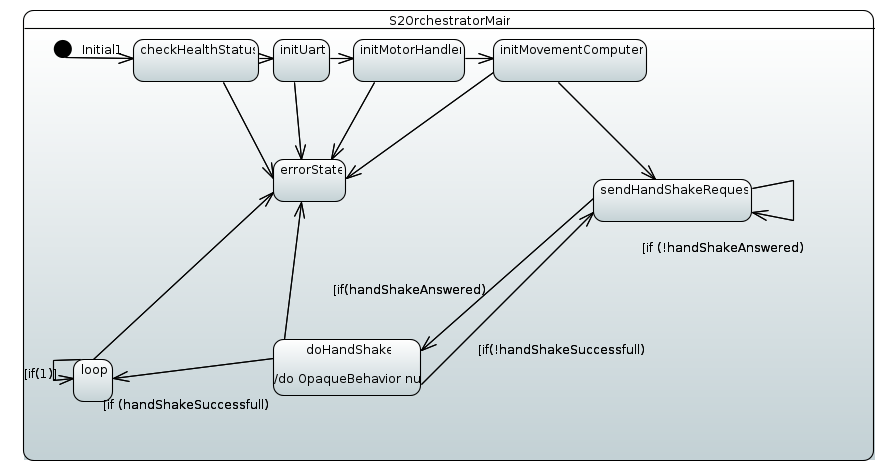
\includegraphics[width=1\linewidth]{pictures/S2OrchestratorMain.PNG}
    \caption{Diagrama de estados del método \texttt{main()} del \textit{orchestrator}.}
    \label{fig:fun_main_orchestrator}
\end{figure}

Este método solo se ejecutará una vez, en cuanto el sistema se ponga en marcha. 

\begin{itemize}
    \item \texttt{checkHealthStatus}: Se verifica la situación de los componentes del brazo robótico para confirmar que todos están en un estado adecuado para el funcionamiento. 
    \item \texttt{initUart}: Se inicializa la UART definiendo una tasa de baudios concreto.
    \item \texttt{initMotorHandler}: Se inicializa el controlador de los motores.
    \item \texttt{initMovementComputer}: Se inicializa el computador de movimientos.
    \item \texttt{sendHandShakeRequest} : Se manda una petición de handshake para verificar si hay algún ordenador conectado. Si se detecta alguno se pasa al siguiente estado, si no, se mantiene en ese estado mandando requests.
    \item \texttt{doHandShake}: Si en el estado anterior se detecta un ordenador se pasa a este estado. Se realiza una serie de intercambios de información para verificar que el ordenador conectado es adecuado para el control del brazo.
    \item \texttt{loop}: Se pasa al bucle de funcionamiento si el handshake ha sido correcto.
    \item \texttt{errorState}: Estado de error al que se llega si en alguno de los estados ocurre algún problema inesperado. 
    
    
\end{itemize}

\begin{figure}[H]
    \centering
    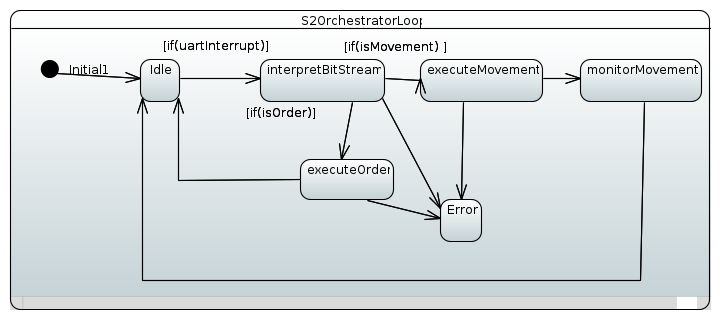
\includegraphics[width=1\linewidth]{pictures/S2OrchestratorLoop.PNG}
    \caption{Diagrama de estados del método \texttt{loop()} del \textit{orchestrator}.}
    \label{fig:fun_loop_orchestrator}
\end{figure}

Este método es el bucle principal del brazo robotico. Tras ejecutar \texttt{main()} el sistema entrará en este bucle y no saldrá hasta que se apaga.

\begin{itemize}
    \item \texttt{Idle}: el brazo se encuentra ocioso y a la espera de una orden desde \ac{S1}
    \item \texttt{interpretBitStream}: tras una interrupción de la UART \ac{S2} entiende que hay una orden o movimiento procedentes de \ac{S1} y se avanza a este estado. La trama de bits es interpretado para saber si es una orden o un movimiento.
    \item \texttt{executeMovement}: si tras interpretar la trama de bits resulta que es un movimiento, el sistema avanza a este estado y se ponen en marcha los demás bloques para poder generar un movimiento en los motores en base a la posición recibida desde \ac{S1}
    \item \texttt{executeOrder}: si tras interpretar la trama de bits resulta que es una orden, el sistema avanza a este estado y se ponen en marcha los bloques necesarios para ejecutar dicha orden.
    \item \texttt{monitorMovement} : tras empezar a ejecutar un movimiento \ac{S2} empieza a monitorizarlo para poder determinar cuando se ha terminado o, si es cancelado, actualizar la posición en la que se ha quedado el brazo.
    \item \texttt{errorState}: Estado de error al que se llega si en alguno de los estados ocurre algún problema inesperado. 
    
    
\end{itemize}

\begin{figure}[H]
    \centering
    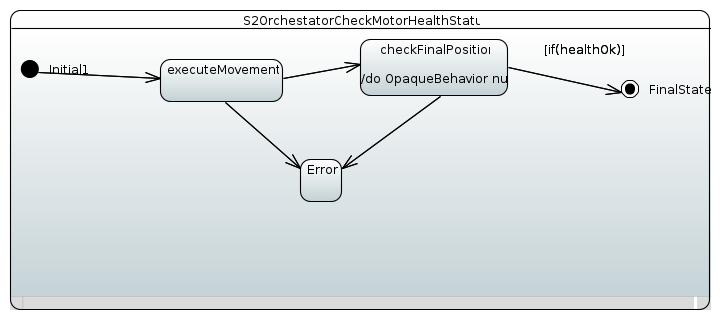
\includegraphics[width=1\linewidth]{pictures/S2OrchestratorCheckMotorHealthStatus.PNG}
    \caption{Diagrama de estados del método \texttt{CheckMotorHealthStatus()} del \textit{orchestrator}.}
    \label{fig:fun_check_motor_health_status_orchestrator}
\end{figure}

Este método comprueba el estado de los motores para asegurar que estos tienen un funcionamiento correcto antes de recibir cualquier orden de movimiento.

\begin{itemize}
    \item \texttt{executeMovement}: se ejecuta un movimiento a una posición en la que todos los fines de carrera sean activados.
    \item \texttt{interpretBitStream}: se verifica que todos los fines de carrera han sido alcanzados pudiendo concluir que el brazo es capaz de mover todos sus motores.
    
\end{itemize}

\begin{figure}[H]
    \centering
    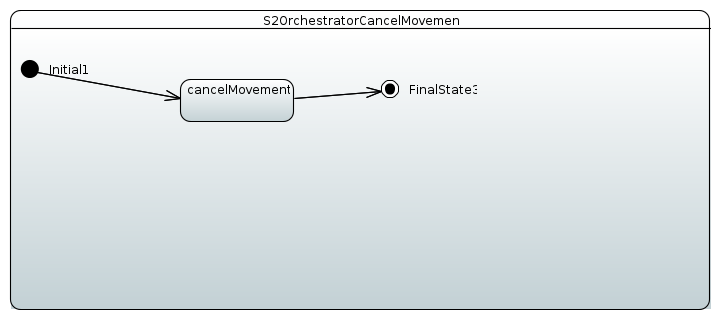
\includegraphics[width=1\linewidth]{pictures/S2OrchestratorCancelMovement.PNG}
    \caption{Diagrama de estados del método \texttt{CancelMovement()} del \textit{orchestrator}.}
    \label{fig:fun_cancel_movement_orchestrator}
\end{figure}

Este método finaliza un movimiento que se este realizando.

\begin{itemize}
    \item \texttt{cancelMovment}: se cancela el movimiento y se guarda la posición actual del brazo.
    
\end{itemize}

\begin{figure}[H]
    \centering
    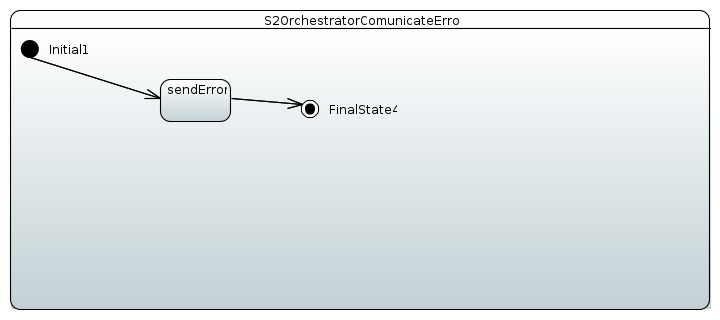
\includegraphics[width=1\linewidth]{pictures/S2OrchestratorComunicateError.PNG}
    \caption{Diagrama de estados del método \texttt{ComunicateError()} del \textit{orchestrator}.}
    \label{fig:fun_comunicate_error_orchestrator}
\end{figure}

Este método comunica un error a \ac{S1}.

\begin{itemize}
    \item \texttt{cancelMovment}: se envía una trama de bits que representa un error ocurrido en \ac{S2}
    
\end{itemize}

\begin{figure}[H]
    \centering
    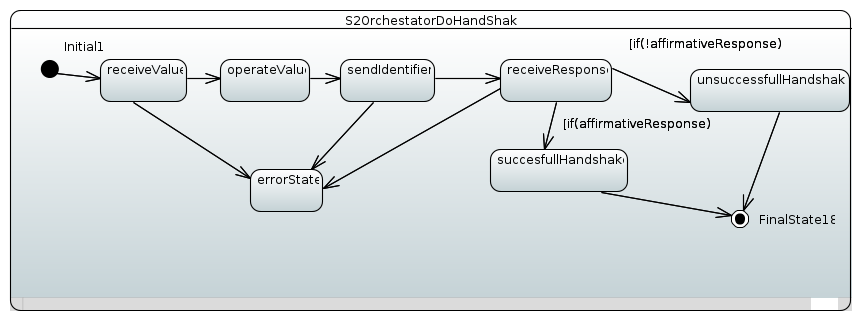
\includegraphics[width=1\linewidth]{pictures/S2OrchestratorDoHandShake.PNG}
    \caption{Diagrama de estados del método \texttt{DoHandShake()} del \textit{orchestrator}.}
    \label{fig:fun_do_hand_shake_orchestrator}
\end{figure}

Este método es el encargado de autenticar a los dispositivos entre si y configurar un canal para su posterior comunicación

\begin{itemize}
    \item \texttt{receiveValue}: se realizan los procedimientos necesarios para recibir un valor desde \ac{S1} a través de la \ac{UART}.
    \item \texttt{operateValue}: se realiza una operación matemática con el valor recibido para generar de esta manera un identificador.
    \item \texttt{sendIdentifier}: se envía dicho identificador de vuelta a \ac{S1}.
    \item \texttt{receiveResponse}: se recibe la respuesta de \ac{S1} para saber si el \textit{hand--shake} ha sido realizado con éxito.
    \item \texttt{succesfulHandshake}: en caso de que en el estado
    \texttt{receiveResponse} se haya recibido una respuesta afirmativa se pasa a este estado que representa que el dispositivo que conforma S1 y S2 han conseguido autenticarse entre si.
    \item \texttt{unsuccesfulHandshake}: en caso de que en el estado \texttt{receiveResponse} se haya recibido una respuesta negativa se pasa a este estado que representa que el dispositivo que conforma S1 y S2 no han conseguido autenticarse
    entre si.
    \item \texttt{errorState}: Estado de error al que se llega si en alguno de los estados ocurre algún problema inesperado. 
\end{itemize}

\begin{figure}[H]
    \centering
    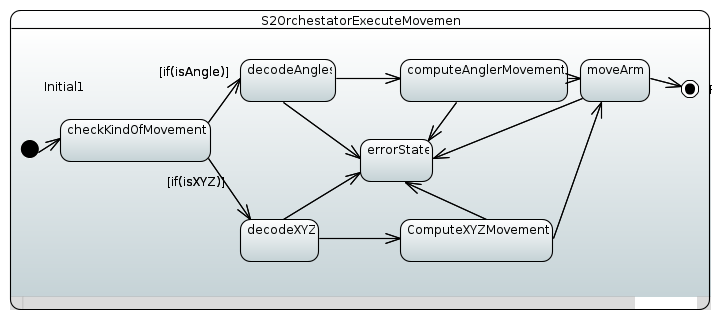
\includegraphics[width=1\linewidth]{pictures/S2OrchestratorExecuteMovement.PNG}
    \caption{Diagrama de estados del método \texttt{ExecuteMovement()} del \textit{orchestrator}.}
    \label{fig:fun_execute_movement_orchestrator}
\end{figure}

Este método es el encargado de, una vez recibida la trama de bits que representa un movimiento desde S1, decidir si el movimiento ha sido representado como ángulos o posiciones cartesianas y posteriormente ordenar las operaciones necesarias para que se generen las señales PWM que moveran los motores.

\begin{itemize}
    \item \texttt{checkKindOfMovement}: Se verifica si el movimiento ha sido transmitido como una posición cartesiana o como unos ángulos destino para los motores y se procede en consecuencia.
    \item \texttt{decodeAngles}: En caso de que fueran ángulos, se transita a este estado. Se interpreta la trama de bits y se obtiene el valor numérico de los ángulos.
    \item \texttt{computeAngleMovement}: Se realizan comprobaciones para verificar que los ángulos están dentro de los limites del brazo y se procede a generar el array de movimientos que se necesitan hacer para conseguir llegar desde la posición actual a la posición destino.
    \item \texttt{decodeXYZ}: En caso de que fueran posiciones cartesianas se transita a este estado. Se interpreta la trama de bits y se obtienen las coordenadas en centímetros.
    \item \texttt{computeXYZMovements}: Para simplificar los cálculos matemáticos posteriores las posiciones cartesianas se convierten en ángulos. Se verifica si los ángulos están dentro de los limites del brazo y se procede a generar el \textit{array} de movimientos que se necesitan hacer para conseguir llegar desde la posición actual a la posición destino.
    \item \texttt{moveArm}: Se envían los movimientos a los motores.
    \item \texttt{errorState}: Estado de error al que se llega si en alguno de los estados ocurre algún problema inesperado. 
    
\end{itemize}

\begin{figure}[H]
    \centering
    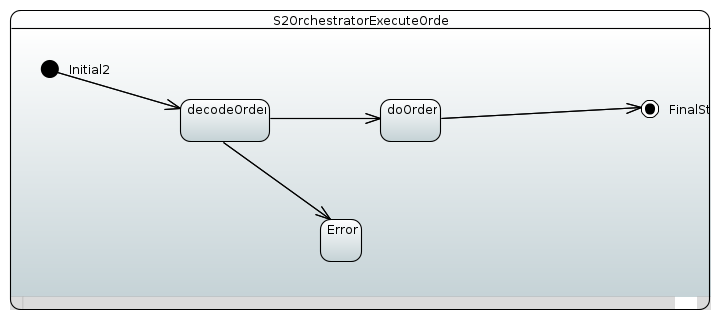
\includegraphics[width=1\linewidth]{pictures/S2OrchestratorExecuteOrder.PNG}
    \caption{Diagrama de estados del método \texttt{ExecuteOrder()} del \textit{orchestrator}.}
    \label{fig:fun_execute_order_orchestator}
\end{figure}

Este método es el encargado de, una vez recibida la trama de bits que representa una orden distinta de realizar un movimiento desde S1, decodificar dicha orden y realizarla.

\begin{itemize}
    \item \texttt{decodeOrder}: Se interpreta la trama de bits para obtener la orden proveniente desde S1.
    \item \texttt{doOrder}: Se ejecuta la orden obtenida en el estado anterior.
    \item \texttt{Error}: Estado de error al que se llega si en alguno de los estados ocurre algún problema inesperado. 
\end{itemize}

\begin{figure}[H]
    \centering
    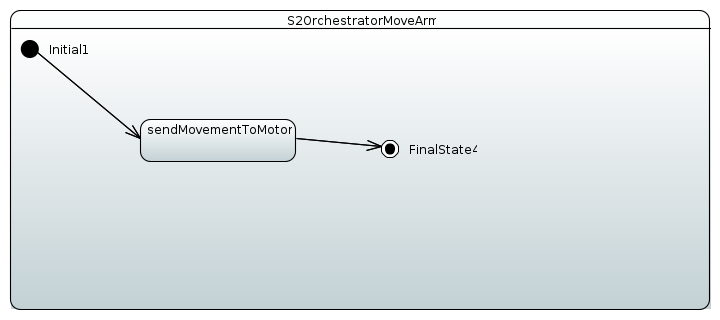
\includegraphics[width=1\linewidth]{pictures/S2OrchestratorMoveArm.PNG}
    \caption{Diagrama de estados del método \texttt{moveArm()} del \textit{orchestrator}.}
    \label{fig:fun_move_arm_orchestator}
\end{figure}

Este método es el encargado de mandar los movimientos a los motores una vez estos se hayan computado.

\begin{itemize}
    \item \texttt{sendMovementToMotors}: se mandan los movimientos necesarios a los motores.
    
\end{itemize}

En el caso del bloque “UART” tenemos los siguientes diagramas.

\begin{figure}[H]
    \centering
    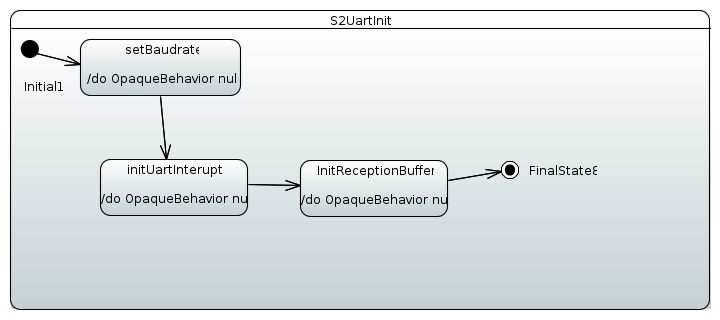
\includegraphics[width=1\linewidth]{pictures/S2UartInit.PNG}
    \caption{Diagrama de estados del método \texttt{uartInit()} del \textit{UART}.}
    \label{fig:fun_uart_init_uart}
\end{figure}

Se ejecuta este método al inicio de la comunicación a través de la UART para configurar la transmisión de datos.

\begin{itemize}
    \item \texttt{setBaudrate}: Se establece una tasa de baudios para la transmisión asíncrona
    \item \texttt{initUartInterupt}: Se configura el registro de interrupciones de tal manera que la UART sea capaz de generar una interrupción en el sistema con el objetivo de poder saber cuando se ha recibido una nueva trama de bits.
    \item \texttt{initReceptionBuffer}: Se inicializa el \textit{buffer} de recepción.
    
\end{itemize}

\begin{figure}[H]
    \centering
    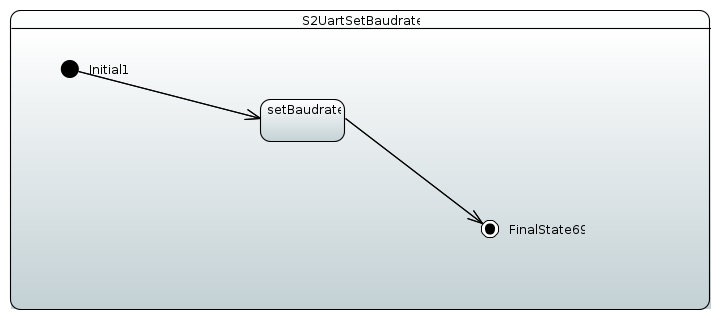
\includegraphics[width=1\linewidth]{pictures/S2UartSetBaudrate.PNG}
    \caption{Diagrama de estados del método \texttt{setBaudrate()} del \textit{UART}.}
    \label{fig:fun_set_baudrate_uart}
\end{figure}

Se configuran los registros necesarios para obtener una tasa de baudios adecuados para la comunicación

\begin{itemize}
    \item \texttt{setBaudrate}: Se realiza la configuración 
\end{itemize}

\begin{figure}[H]
    \centering
    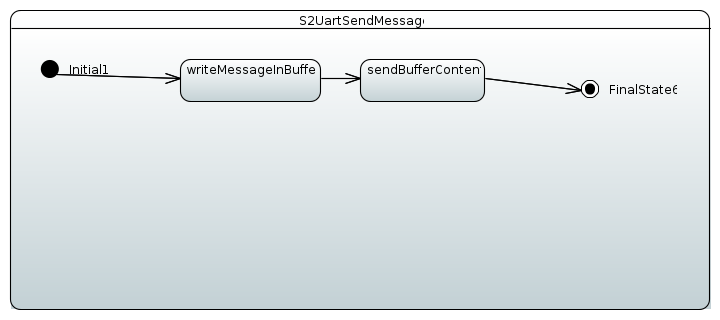
\includegraphics[width=1\linewidth]{pictures/S2UartSendMessage.PNG}
    \caption{Diagrama de estados del método \texttt{sendMessage()} del \textit{UART}.}
    \label{fig:fun_send_message_uart}
\end{figure}

Se escribe un mensaje en el \textit{buffer} de envio y este es posteriormente enviado.

\begin{itemize}
    \item \texttt{writeMessageInBuffer}: Se escribe el mensaje en el \textit{buffer} de salida de la UART.
    \item \texttt{sendBufferContent}: Se envía el contenido del buffer a \ac{S1}
\end{itemize}

\begin{figure}[H]
    \centering
    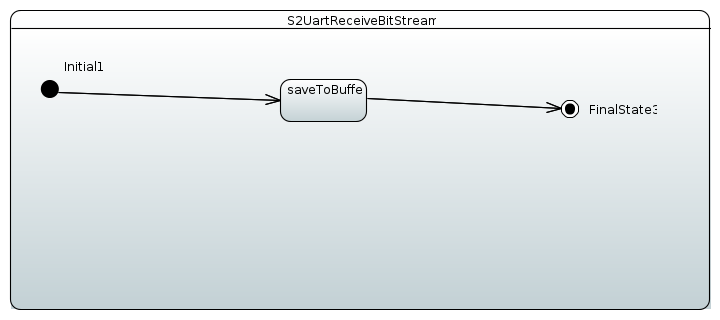
\includegraphics[width=1\linewidth]{pictures/S2UartReceiveBitStream.PNG}
    \caption{Diagrama de estados del método \texttt{receiveBitStream()} del \textit{UART}.}
    \label{fig:fun_receive_bit_stream_uart}
\end{figure}

Se guarda un mensaje en el \textit{buffer} de recepción.

\begin{itemize}
    \item \texttt{saveToBuffer}: Se escribe el mensaje en el \textit{buffer} de entrada de la UART.
\end{itemize}


En el caso del bloque “MotorHandler” tenemos los siguientes diagramas.

\begin{figure}[H]
    \centering
    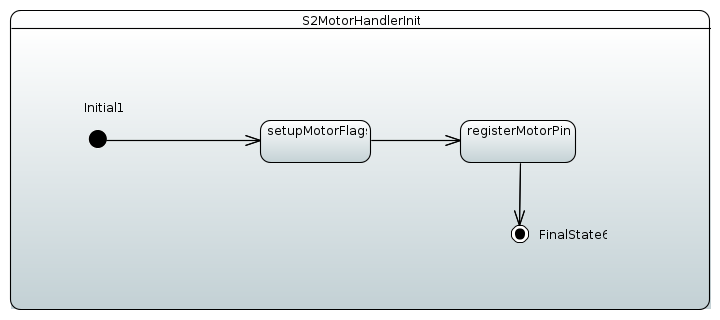
\includegraphics[width=1\linewidth]{pictures/S2MotorHandlerInit.PNG}
    \caption{Diagrama de estados del método \texttt{init()} del \textit{motorHandler}.}
    \label{fig:fun_init_motor_handler}
\end{figure}

Se inicializan los \textit{flags} y se registran los pines a los que están conectados los motores

\begin{itemize}
    \item \texttt{setupMotorFlags}: Se establecen los flags de los motores.
    \item \texttt{registerMotorPin}: Se registran los pines físicos a los que están conectados los motores con el objetivo de saber donde se deben enviar las señales PWM.
\end{itemize}

\begin{figure}[H]
    \centering
    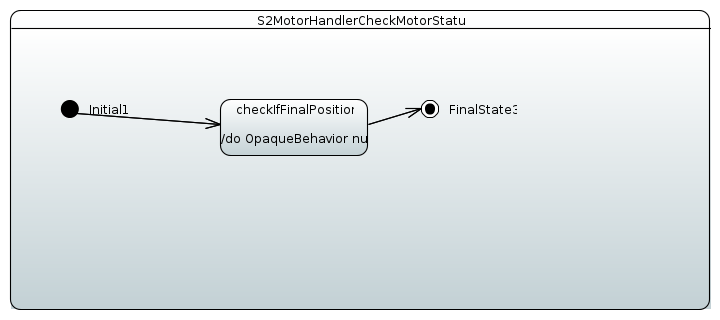
\includegraphics[width=1\linewidth]{pictures/S2MotorHandlerCheckMotorStatus.PNG}
    \caption{Diagrama de estados del método \texttt{checkMotorStatus()} del \textit{motorHandler}.}
    \label{fig:fun_check_motor_status_motor_handler}
\end{figure}

Este método sirve para asegurar que los motores están en buenas condiciones de funcionamiento

\begin{itemize}
    \item \texttt{checkIfFinalPosition}: Se envía a los motores a una posición en la que se sabe que debería estar en contacto con algún fin de carrera y posteriormente se verifica que dichos fines de carrera están activados. De esta manera se asegura que los motores pueden girar.

\end{itemize}

\begin{figure}[H]
    \centering
    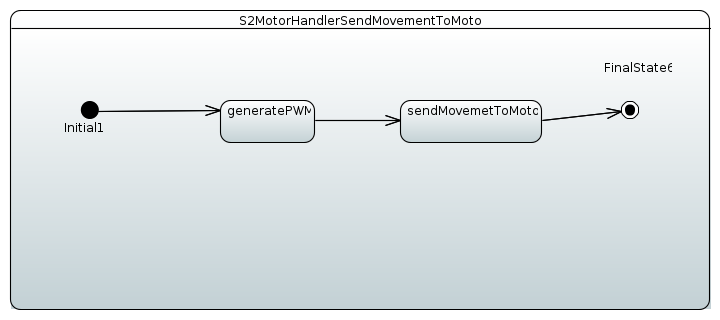
\includegraphics[width=1\linewidth]{pictures/S2MotorHandlerSendMovementToMotors.PNG}
    \caption{Diagrama de estados del método \texttt{sendMovementToMotors()} del \textit{motorHandler}.}
    \label{fig:fun_send_movement_to_motors_motor_handler}
\end{figure}

Se genera una señal PWM y se envia al motor correspondiente

\begin{itemize}
    \item \texttt{generatePWM}: En base al \textit{array} de movimientos que se obtiene a través del \textit{orchestator} y del \textit{movementComputer} se generar las señales PWM necesarias para poder realizarlos.
    
    \item \texttt{sendMovementToMotor}: Se envia la seña PWM al motor.

\end{itemize}

\begin{figure}[H]
    \centering
    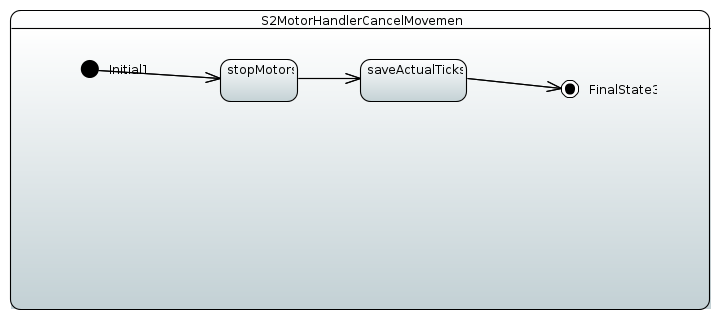
\includegraphics[width=1\linewidth]{pictures/S2MotorHandlerCancelMovement.PNG}
    \caption{Diagrama de estados del método \texttt{cancelMovement()} del \textit{motorHandler}.}
    \label{fig:fun_cancel_movement_motor_handler}
\end{figure}

Se cancela un movimiento que se este ejecutando actualmente

\begin{itemize}
    \item \texttt{stopMotor}: Se para el motor.
    \item \texttt{saveActualTicks}: Se guardan los ticks actuales que el motor ha recorrido. Los \textit{ticks} representan ciclos de instrucción durante los cuales el motor recibe una señal PWM especifica. Se entra en detalle sobre este aspecto en apartados posteriores del documento.

\end{itemize}

En el caso del bloque “MovementComputer” tenemos los siguientes diagramas:

\begin{figure}[H]
    \centering
    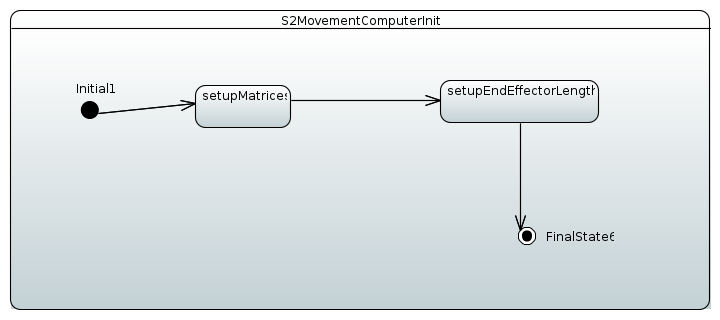
\includegraphics[width=1\linewidth]{pictures/S2MovementComputerInit.PNG}
    \caption{Diagrama de estados del método \texttt{init()} del \textit{movementComputer}.}
    \label{fig:fun_init_movement_computer}
\end{figure}

Se inicializan las matrices de la cinemática directa e inversa y se define la distancia del \textit{end--effector} desde la base del brazo.

\begin{itemize}
    \item \texttt{setupMatrices}: Se inicializan las matrices de la cinemática directa e inversa.
    \item \texttt{setupEndEffectorLength}: Se definen la distancia desde la base hasta el \textit{end--effector}.
\end{itemize}

\begin{figure}[H]
    \centering
    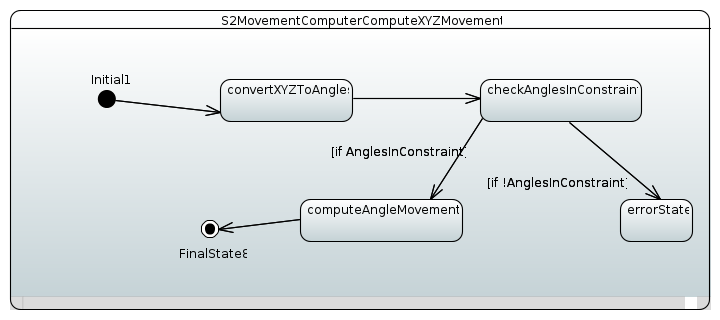
\includegraphics[width=1\linewidth]{pictures/S2MovementComputerComputeXYZMovement.PNG}
    \caption{Diagrama de estados del método \texttt{computeXYZMovement()} del \textit{movementComputer}.}
    \label{fig:fun_compute_xyz_movement_movement_computer}
\end{figure}

\begin{itemize}
    \item \texttt{convertXYZToAngles}: Se emplea la cinemática inversa para obtener la posición de los motores a partir de la posición del \textit{end--effector}
    \item \texttt{checkAnglesInContraint}: Se verifica si los ángulos están dentro de las limitaciones de los motores.
    \item \texttt{computeAngleMovement}: Se calcula el movimiento que se debe realizar para mover el \textit{end--effector} desde la posicion actual a la deseada.
    \item \texttt{errorState}: Estado de error al que se llega si en alguno de los estados ocurre algún problema inesperado. 
\end{itemize}

\begin{figure}[H]
    \centering
    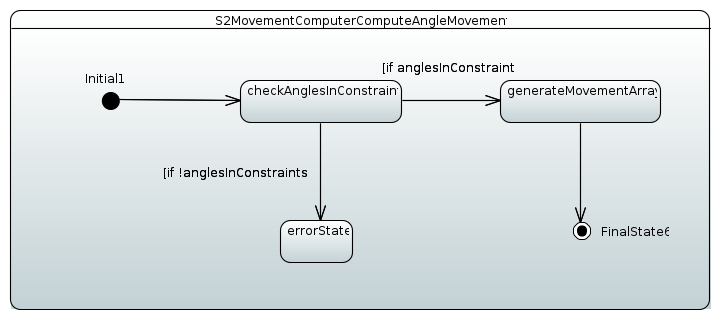
\includegraphics[width=1\linewidth]{pictures/S2MovementComputerComputeAngleMovement.PNG}
    \caption{Diagrama de estados del método \texttt{computeAngleMovement()} del \textit{movementComputer}.}
    \label{fig:fun_compute_angle_mocement_movement_computer}
\end{figure}

\begin{itemize}
    \item \texttt{checkAnglesInContraint}: Se verifica si los ángulos están dentro de las limitaciones de los motores.
    \item \texttt{generateMovementArray}: Se generan los array de movimientos.
    \item \texttt{errorState}: Estado de error al que se llega si en alguno de los estados ocurre algún problema inesperado. 
\end{itemize}